\documentclass[conference]{IEEEtran}
\usepackage[utf8]{inputenc}
\usepackage[T1]{fontenc}
\usepackage[spanish,es-tabla]{babel}
\usepackage{graphicx}
\usepackage{booktabs}
\usepackage{amsmath}
\usepackage{url}
\usepackage{microtype}
\graphicspath{{../resultados/figuras/}}
\begin{document}
\title{Clasificación de tumores de mama con Naive Bayes, SVM y una red neuronal}
\author{\IEEEauthorblockN{Jose Antonio Ortega Jacobo}
\IEEEauthorblockA{CU UAEMEX Texcoco\\Ingeniería en Computación}}
\maketitle
\begin{abstract}
En este proyecto se trabajó con un conjunto de datos de características de tumores de mama para practicar la clasificación supervisada. El objetivo fue comparar tres modelos vistos en el curso: Naive Bayes, máquinas de soporte vectorial (SVM) y una red neuronal. También se entrenó una regresión logística para tener un punto de comparación. Se usaron 569 registros y 30 variables numéricas del conjunto Breast Cancer Wisconsin (Diagnostic). Primero se revisaron los datos y se realizaron gráficas para conocer sus distribuciones y correlaciones. Después se dividieron los registros en entrenamiento, validación y prueba; se escalaron las variables sin utilizar información de la prueba y se buscaron parámetros mediante validación cruzada de cinco partes. Para evaluar se utilizaron exactitud, precisión, sensibilidad, F1, matrices de confusión y curvas ROC. En los datos de prueba, la regresión logística y SVM obtuvieron 98.25\,\% de exactitud y 0.9756 de F1. Los resultados muestran que un modelo sencillo puede funcionar tan bien como uno más elaborado en este conjunto. El ejercicio tiene fines académicos y no reemplaza una valoración médica.
\end{abstract}
\begin{IEEEkeywords}
ciencia de datos, clasificación, cáncer de mama, Naive Bayes, SVM, red neuronal.
\end{IEEEkeywords}

\section{Introducción}
En ciencia de datos, la clasificación consiste en usar ejemplos que ya tienen una respuesta conocida para aprender a clasificar casos nuevos. En este trabajo se busca distinguir entre dos clases: tumor benigno y tumor maligno. Es un ejemplo útil para la materia porque tenemos varias características numéricas y una respuesta conocida para cada registro.

El propósito no es crear una aplicación médica. El objetivo es seguir los pasos básicos de un proyecto de ciencia de datos: cargar la información, revisar los datos, prepararlos, entrenar modelos y comparar resultados. Se eligió el conjunto Breast Cancer Wisconsin (Diagnostic), conocido también como WDBC, porque es público, pequeño y permite trabajar en una computadora normal.

Se compararon cuatro modelos. Los tres principales fueron Naive Bayes, SVM y una red neuronal de tipo perceptrón multicapa. Se agregó una regresión logística como modelo de referencia. Para que la comparación fuera justa, todos trabajaron con la misma división de datos y con las mismas métricas.

\section{Trabajo relacionado}
El conjunto de datos se relaciona con el trabajo de Wolberg, Street y Mangasarian sobre la clasificación de tumores a partir de mediciones celulares \cite{wolberg}. Para este proyecto se utilizó una copia disponible en \texttt{scikit-learn}, correspondiente al conjunto del repositorio UCI.

Naive Bayes es un método que utiliza probabilidades. Rish estudió su funcionamiento y sus ventajas como clasificador sencillo \cite{rish}. Una de sus suposiciones es que las características se comportan de forma independiente dentro de cada clase, algo que aquí no se cumple completamente porque hay variables muy correlacionadas.

Cortes y Vapnik describieron las máquinas de soporte vectorial \cite{cortes}. Estos modelos buscan una separación entre clases. Se pueden probar distintas formas de separación, por ejemplo lineal y RBF. Para la red neuronal se tomó como antecedente el trabajo sobre aprendizaje mediante retropropagación de Rumelhart, Hinton y Williams \cite{rumelhart}. Finalmente, Fawcett explicó el uso de las curvas ROC como una forma de comparar clasificadores \cite{fawcett}. Estas cinco referencias son las que se utilizaron para entender las partes principales del proyecto.

\section{Datos y análisis exploratorio}
\subsection{Descripción del conjunto}
El conjunto tiene \textbf{569 filas y 30 características numéricas}. Hay 357 registros benignos y 212 malignos. Entre las características aparecen el radio, textura, perímetro, área y concavidad de los núcleos celulares. Los valores no son imágenes; son números obtenidos de las imágenes originales.

Se revisó la cantidad de registros, los tipos de datos, las filas repetidas y los valores faltantes. No se encontraron valores faltantes ni registros repetidos en las características. Tampoco fue necesario convertir textos a números, porque todas las columnas utilizadas para entrenar son numéricas.

En la copia de \texttt{scikit-learn}, el valor 0 significa maligno y el 1 significa benigno. Para facilitar la interpretación se cambiaron las etiquetas: en el proyecto \textbf{1 significa maligno} y \textbf{0 significa benigno}. Así, la sensibilidad indica cuántos casos malignos fueron detectados.


\subsection{Primera revisión con Python}
Antes de entrenar, se imprimieron el tamaño del conjunto, las primeras filas, la cantidad de valores faltantes y la cantidad de diagnósticos de cada tipo. Estas tareas se pueden hacer con funciones básicas de \texttt{pandas}, por ejemplo \texttt{head()}, \texttt{shape}, \texttt{isna()} y \texttt{value\_counts()}. En este caso se utilizó \texttt{load\_breast\_cancer()} para cargar los datos, pero después se trabajó con un \texttt{DataFrame} normal.

Un aspecto que llamó la atención es que las 30 columnas vienen de diez mediciones distintas. Para cada medición hay una media, un error estándar y un valor extremo. Por ejemplo, existen tres columnas relacionadas con el radio. Esto explica por qué varios atributos pueden aportar información parecida. El hecho de tener 30 columnas no significa necesariamente que las 30 sean independientes entre sí.

En el EDA no se intentó adivinar qué algoritmo iba a ganar. El objetivo fue comprender cómo están distribuidos los registros y si era necesario limpiar algo. Se revisaron valores faltantes y repetidos y se comprobaron las proporciones de ambas clases. Los resultados de esta revisión se muestran en las gráficas siguientes. Como el conjunto tiene más benignos que malignos, también se decidió incluir sensibilidad y F1 en la evaluación.

\subsection{Gráficas del EDA}
El análisis exploratorio se hizo con los datos de entrenamiento para no utilizar información de prueba al tomar decisiones. La Fig.~\ref{fig:clases} presenta la cantidad de casos de cada diagnóstico. Hay más casos benignos; por esa razón, no conviene revisar solamente la exactitud.

\begin{figure}[!t]
\centering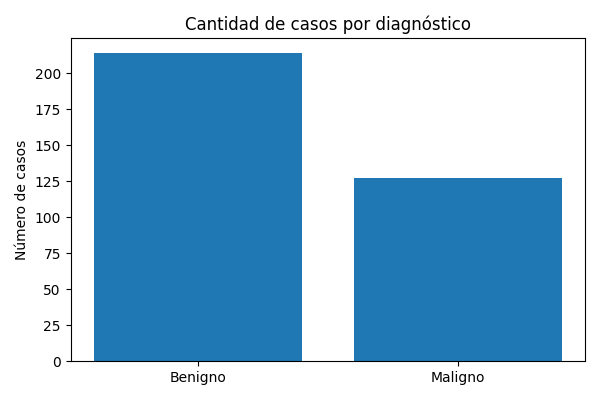
\includegraphics[width=.87\linewidth]{01_clases.png}
\caption{Cantidad de casos benignos y malignos en entrenamiento.}
\label{fig:clases}
\end{figure}

En la Fig.~\ref{fig:radio} se muestra un histograma del radio medio. Muchos casos malignos presentan valores más altos, aunque hay una zona donde se mezclan los dos grupos. Esto indica que el radio ayuda, pero no basta para clasificar todos los casos.

\begin{figure}[!t]
\centering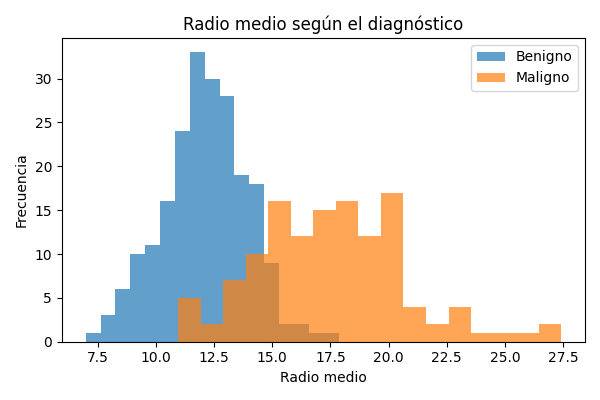
\includegraphics[width=.89\linewidth]{02_radio_hist.png}
\caption{Histograma del radio medio de los dos diagnósticos.}
\label{fig:radio}
\end{figure}

La Fig.~\ref{fig:corr} es un mapa de correlaciones de diez variables. Algunas están muy relacionadas: por ejemplo, el radio medio y el perímetro medio tienen una correlación cercana a 0.998. Esto es importante al interpretar Naive Bayes, que trabaja con una suposición de independencia entre características.

\begin{figure}[!t]
\centering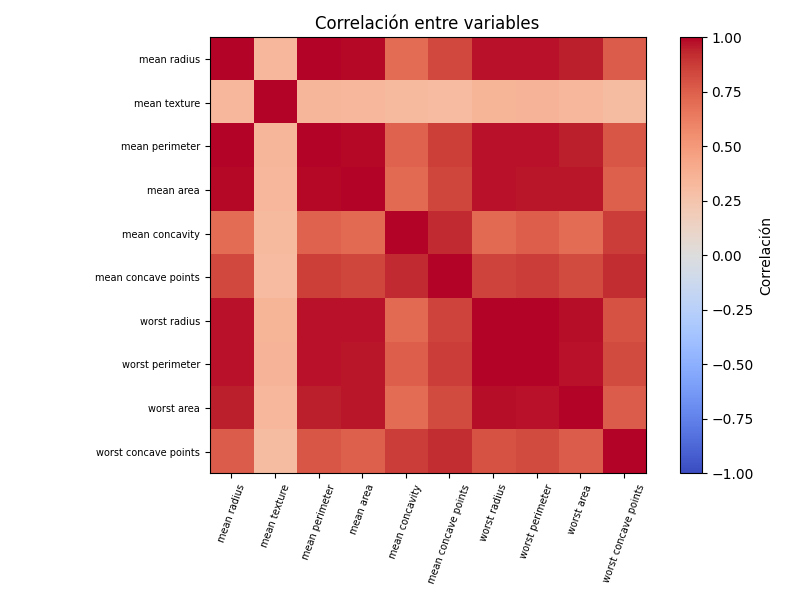
\includegraphics[width=.92\linewidth]{03_correlaciones.png}
\caption{Correlaciones de diez variables del conjunto de entrenamiento.}
\label{fig:corr}
\end{figure}

La Fig.~\ref{fig:cajas} compara los puntos cóncavos extremos con un diagrama de caja. Aunque las medianas de los dos grupos son distintas, los valores no están totalmente separados. Por eso se utilizan las 30 características en el entrenamiento.

\begin{figure}[!t]
\centering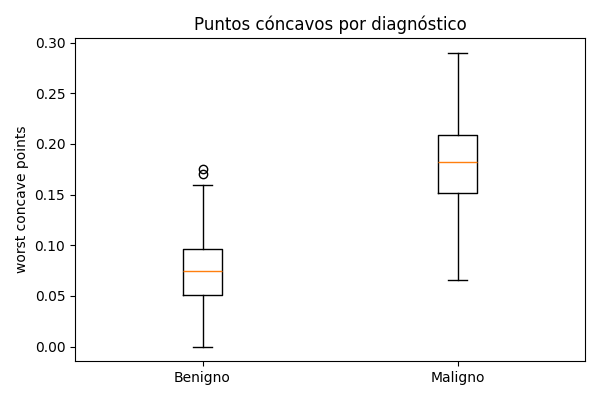
\includegraphics[width=.89\linewidth]{04_boxplot.png}
\caption{Diagrama de caja de puntos cóncavos según el diagnóstico.}
\label{fig:cajas}
\end{figure}


\subsection{Interpretación de las gráficas}
Las gráficas permiten responder preguntas diferentes. El conteo de clases nos dice con qué frecuencia aparece cada etiqueta. El histograma de radio permite comparar una variable concreta. El diagrama de caja resume dónde se concentran los valores y cuáles parecen más altos o bajos. Finalmente, el mapa de correlaciones ayuda a identificar columnas que cambian de manera parecida.

Por ejemplo, si el radio y el perímetro son altos en un registro, no se deben contar necesariamente como dos evidencias totalmente independientes. Los modelos trabajan con las variables de manera distinta: Naive Bayes tiene una suposición de independencia, mientras que SVM y la red neuronal pueden aprender combinaciones de características. Esta diferencia hace interesante la comparación. Sin embargo, el EDA por sí solo no demuestra que un modelo vaya a funcionar mejor; eso debe revisarse con datos separados.

\section{Preparación y modelos}
\subsection{División y escalado}
Se utilizó la semilla 42 para repetir la misma separación: \textbf{341 filas para entrenamiento}, \textbf{114 para validación} y \textbf{114 para prueba}. Se usó una división estratificada, es decir, se conservó aproximadamente la proporción de benignos y malignos en los tres grupos.

Las variables tienen distintas escalas: algunas miden tamaños y otras tienen valores pequeños. Por eso se utilizó \texttt{StandardScaler}, especialmente necesario para SVM y para la red neuronal. Se colocó el escalador y el modelo dentro de un \texttt{Pipeline}. De este modo, la media y la desviación del escalado se calculan solo con los datos usados para entrenar cada vez. Esto evita mezclar información del conjunto de prueba con el entrenamiento.


\subsection{Por qué separar los datos}
La división se hizo antes de entrenar y también antes de calcular las gráficas que podrían orientar el análisis. Los 341 registros de entrenamiento se usaron para ajustar los modelos y para buscar sus mejores parámetros. Los 114 de validación sirvieron para comparar los modelos ya entrenados, y los 114 de prueba quedaron apartados para la evaluación final.

Se usó \texttt{train\_test\_split} dos veces para conseguir las proporciones 60\,\%, 20\,\% y 20\,\%. Con \texttt{random\_state=42} se obtiene la misma división cuando otra persona ejecuta el código. Con \texttt{stratify} se mantiene un porcentaje parecido de clases en las tres partes. Esto evita que una separación al azar deje muy pocos ejemplos malignos en alguno de los conjuntos.

También fue importante hacer el escalado dentro de cada entrenamiento. Si se calcularan las medias y desviaciones con todas las filas desde el inicio, el modelo ya habría utilizado información de prueba sin querer. El uso de \texttt{Pipeline} resuelve esa parte automáticamente, incluso durante la validación cruzada. Aunque el nombre parece avanzado, en el código solo indica que se hacen dos pasos seguidos: escalar los números y entrenar el modelo.

\subsection{Modelos utilizados}
Se trabajó con los siguientes modelos:\par
\textbf{Regresión logística:} se usó como punto de comparación. Es un modelo relativamente sencillo que funciona bien como referencia para clasificación binaria.\par
\textbf{Naive Bayes:} se usó \texttt{GaussianNB} porque las variables son numéricas. Supone que cada característica tiene una distribución aproximadamente normal dentro de su clase y que las características son independientes al conocer la clase; esta última suposición no se cumple por completo.\par
\textbf{SVM:} se probaron el kernel lineal y RBF. También se probaron diferentes valores de $C$ y $\gamma$, que cambian la forma en que el modelo separa las clases.\par
\textbf{Red neuronal:} se utilizó \texttt{MLPClassifier}, con una o dos capas ocultas pequeñas y activación ReLU. Se probaron distintos valores de $\alpha$ como regularización para reducir el sobreajuste.


El clasificador de referencia permite tener un punto de partida. Si un modelo con más opciones no mejora el resultado, no es obligatorio escoger el más complicado. En Naive Bayes se probaron pequeños cambios al parámetro \texttt{var\_smoothing}, que sirve para trabajar de forma más estable con las varianzas. Para SVM se comparó una línea de separación con una frontera no lineal RBF. En la red neuronal se probaron pocas neuronas, en lugar de crear una arquitectura demasiado grande para 569 registros.

La red neuronal utilizó penalización L2 mediante el parámetro \texttt{alpha}. La idea es evitar que los pesos tomen valores demasiado grandes y que el modelo se ajuste excesivamente a los ejemplos de entrenamiento. No se usaron herramientas adicionales como redes profundas o procesamiento de imágenes, porque el conjunto ya contiene los números listos para aprender.

Los parámetros se probaron con \texttt{GridSearchCV} y cinco divisiones de validación cruzada. Esto significa que el programa ensaya varias opciones y compara su F1 promedio antes de elegir los mejores parámetros. El espacio utilizado se muestra en la Tabla~\ref{tab:param}.

\begin{table}[!t]
\centering
\caption{Parámetros probados en cada modelo}
\label{tab:param}
\footnotesize
\begin{tabular}{p{.28\linewidth}p{.64\linewidth}}
\toprule
Modelo & Valores probados\\\midrule
Reg. logística & $C$: 0.1, 1, 10\\
Naive Bayes & \texttt{var\_smoothing}: $10^{-10}$, $10^{-9}$, $10^{-8}$, $10^{-7}$\\
SVM lineal & $C$: 0.1, 1, 10\\
SVM RBF & $C$: 0.1, 1, 10; $\gamma$: 0.01, 0.1, 1, \texttt{scale}\\
Red neuronal & Capas: (16), (32), (32,16); $\alpha$: 0.001, 0.01, 0.1\\
\bottomrule
\end{tabular}
\end{table}

En total se ensayaron 31 combinaciones de parámetros. Se utilizó F1 como criterio para buscar una opción que mantuviera tanto precisión como sensibilidad. Los datos de validación se emplearon para elegir el modelo preferido y los datos de prueba solo para realizar la comparación final.

\section{Experimentos y resultados}
\subsection{Resultados de validación cruzada}
La Tabla~\ref{tab:cv} muestra el F1 promedio de cinco divisiones y la desviación estándar. La desviación ayuda a saber cuánto cambia el resultado según los datos que se usaron para entrenar y validar. SVM, red neuronal y regresión logística tuvieron resultados cercanos. Naive Bayes quedó por debajo de los demás.

\begin{table}[!t]
\centering
\caption{F1 promedio y variación en validación cruzada}
\label{tab:cv}
\footnotesize
\begin{tabular}{lcc}
\toprule Modelo & F1 promedio & Desv. estándar\\\midrule
Reg. logística & 0.9636 & 0.0276\\
Naive Bayes & 0.8886 & 0.0520\\
SVM & 0.9637 & 0.0266\\
Red neuronal & 0.9631 & 0.0331\\
\bottomrule
\end{tabular}
\end{table}

\begin{figure}[!t]
\centering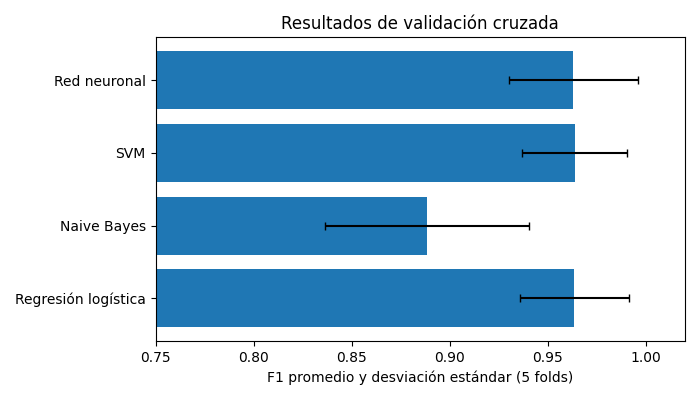
\includegraphics[width=.92\linewidth]{08_cv_variabilidad.png}
\caption{Promedio y variación de F1 en cinco divisiones.}
\label{fig:cv}
\end{figure}

La Fig.~\ref{fig:cv} representa los mismos valores de manera gráfica. Como las diferencias de F1 entre los tres mejores modelos son pequeñas comparadas con sus desviaciones, no es correcto asegurar que uno sea superior en general. En la partición de validación independiente, regresión logística obtuvo F1 de 0.9762 y se seleccionó como modelo de referencia para la discusión.


\subsection{Revisión con validación independiente}
Después de elegir los parámetros con validación cruzada, cada mejor modelo se probó con las 114 filas de validación. Esta prueba intermedia es diferente de la validación cruzada: se realiza en datos que no participaron en el ajuste de cada modelo. Su objetivo fue elegir cuál se tomaría como primera opción antes de ver los resultados finales.

\begin{table}[!t]
\centering
\caption{Métricas obtenidas en validación independiente}
\label{tab:val}
\footnotesize
\begin{tabular}{lccc}
\toprule Modelo & Exactitud & Sensibilidad & F1\\\midrule
Reg. logística & .9825 & .9535 & .9762\\
Naive Bayes & .9561 & .9302 & .9412\\
SVM & .9737 & .9767 & .9655\\
Red neuronal & .9737 & .9767 & .9655\\
\bottomrule
\end{tabular}
\end{table}

Según la Tabla~\ref{tab:val}, la regresión logística tuvo el F1 más alto en validación. SVM y la red neuronal tuvieron una sensibilidad ligeramente mayor, pero un F1 menor. Esto no quiere decir que las diferencias sean muy grandes; solamente indica cuál modelo resultó mejor de acuerdo con el criterio establecido para esta separación de datos.

\subsection{Resultados finales de prueba}
Después de elegir los parámetros se revisaron las 114 filas de prueba, que no se habían usado para entrenar. La Tabla~\ref{tab:test} reúne las métricas solicitadas. Aquí, precisión significa qué porcentaje de las predicciones de maligno fue correcto, y sensibilidad significa qué porcentaje de los malignos reales fue detectado. F1 combina ambas métricas.

\begin{table}[!t]
\centering
\caption{Comparación de modelos en los datos de prueba}
\label{tab:test}
\scriptsize
\begin{tabular}{lccccc}
\toprule Modelo & Exact. & Prec. & Sens. & F1 & AUC\\\midrule
Reg. logística & .9825 & 1.0000 & .9524 & .9756 & .9977\\
Naive Bayes & .9211 & .9231 & .8571 & .8889 & .9897\\
SVM & .9825 & 1.0000 & .9524 & .9756 & .9957\\
Red neuronal & .9561 & .9512 & .9286 & .9398 & .9894\\
\bottomrule
\end{tabular}
\end{table}


Para interpretar las métricas, primero se revisó la matriz de confusión. Un verdadero positivo (VP) es un tumor maligno que el modelo predice como maligno. Un falso negativo (FN) es maligno, pero el modelo lo predice como benigno. Un falso positivo (FP) es benigno, pero se predice como maligno. Un verdadero negativo (VN) es benigno y se clasifica correctamente. A partir de esos cuatro conteos se calculan las métricas:
\begin{equation}
\text{Precisión}=\frac{VP}{VP+FP},\quad
\text{Sensibilidad}=\frac{VP}{VP+FN}.
\end{equation}
\begin{equation}
F1=\frac{2\,(\text{Precisión})\,(\text{Sensibilidad})}{\text{Precisión}+\text{Sensibilidad}}.
\end{equation}
La exactitud es la cantidad total de aciertos dividida entre la cantidad de registros. AUC resume qué tan bien se ordenan los puntajes del clasificador en distintos umbrales. Estas métricas se usaron juntas porque un solo número no describe todos los tipos de error.

La regresión logística y SVM clasificaron correctamente 112 de los 114 casos, por lo que tuvieron 98.25\,\% de exactitud. También obtuvieron el mismo F1. La red neuronal quedó un poco por debajo y Naive Bayes tuvo la sensibilidad más baja. Este último resultado indica que dejó sin detectar más casos malignos.

La matriz de confusión permite ver los errores por clase. En la Fig.~\ref{fig:matriz} se observan dos falsos negativos para regresión logística y SVM; es decir, dos casos malignos fueron clasificados como benignos. En cambio, Naive Bayes presentó seis falsos negativos y tres falsos positivos.

\begin{figure}[!t]
\centering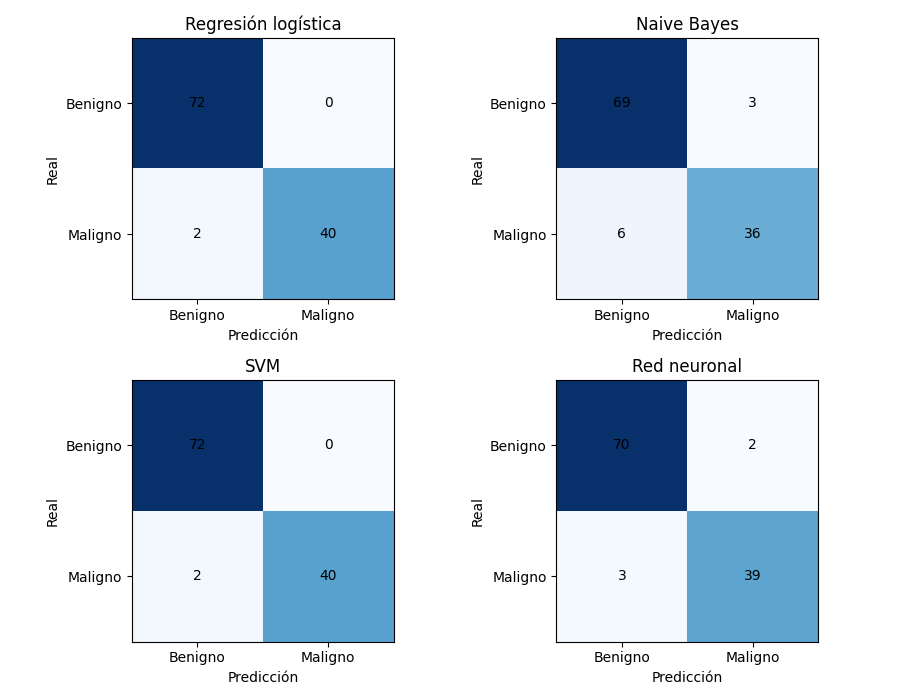
\includegraphics[width=.97\linewidth]{05_matrices_confusion.png}
\caption{Matrices de confusión de los cuatro modelos.}
\label{fig:matriz}
\end{figure}

Las curvas ROC de la Fig.~\ref{fig:roc} sirven para observar qué tan bien los modelos separan las dos clases a diferentes umbrales. Sus áreas bajo la curva son elevadas, aunque eso no significa que no haya errores. La Fig.~\ref{fig:pr} presenta además las curvas precisión-recall, importantes porque existen más casos benignos que malignos.

\begin{figure}[!t]
\centering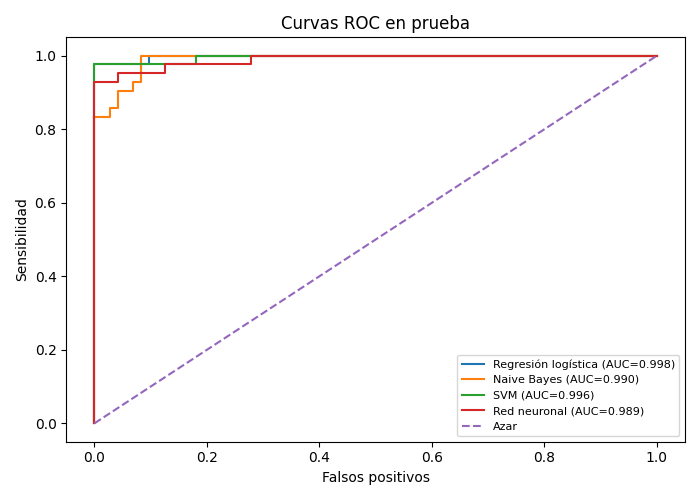
\includegraphics[width=.91\linewidth]{06_roc.png}
\caption{Curvas ROC construidas con los datos de prueba.}
\label{fig:roc}
\end{figure}
\begin{figure}[!t]
\centering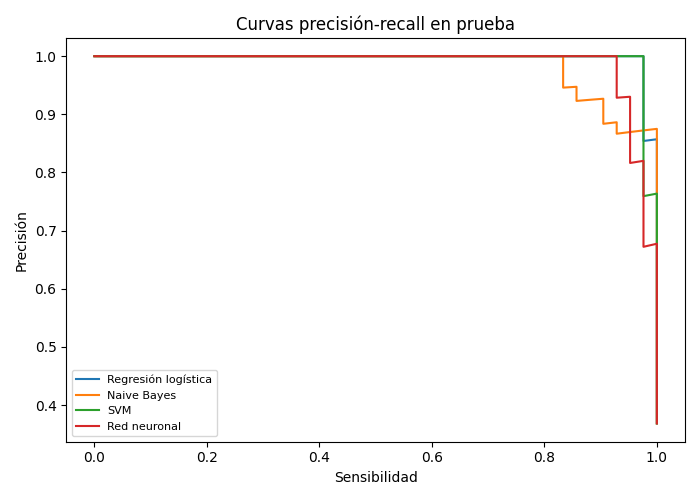
\includegraphics[width=.91\linewidth]{07_precision_recall.png}
\caption{Curvas precisión-recall de los cuatro modelos.}
\label{fig:pr}
\end{figure}

\subsection{Revisión de errores}
Para revisar los errores se guardó un archivo CSV con los registros mal clasificados. En regresión logística y SVM se repitieron los casos con índices 73 y 205. Ambos eran malignos, pero fueron predichos como benignos. Sus valores de radio medio y puntos cóncavos se encuentran en zonas que pueden parecerse a las de otros registros benignos. Esto podría explicar parte de la confusión, aunque no permite asegurar la causa exacta.

La red neuronal produjo tres falsos negativos y dos falsos positivos. Naive Bayes cometió más errores, posiblemente porque varias mediciones están relacionadas y su supuesto de independencia no describe completamente los datos. Aunque una exactitud de 98\,\% parece alta, los falsos negativos deben revisarse por separado, especialmente cuando la clase positiva representa tumores malignos.

\section{Discusión}
Los resultados muestran que la regresión logística y SVM se comportaron de manera muy parecida. Esto indica que un modelo sencillo puede obtener resultados comparables a uno más complejo con estos datos. No significa que siempre sea mejor, porque el conjunto es pequeño y solo se probó una separación final de los datos.

Naive Bayes fue el más simple de configurar, pero presentó el F1 más bajo. Una posible razón es la relación entre algunas variables. SVM consiguió buenos resultados al probar el kernel lineal y RBF; el mejor fue RBF con $C=10$ y $\gamma=0.01$. En la red neuronal, la búsqueda seleccionó una capa oculta de 32 neuronas y $\alpha=0.1$; la regularización se usó para disminuir el riesgo de que memorizara los ejemplos.

Esta comparación tiene limitaciones. El conjunto de 569 casos no representa a todos los pacientes y no se utilizaron datos de otro hospital para comprobar los resultados. La validación cruzada se hizo sobre una partición y la evaluación final contiene solo 114 muestras. El estudio sirve para practicar métodos de clasificación, pero no para hacer diagnósticos médicos reales.


\section{Reproducibilidad del ejercicio}
El proyecto se organizó de forma que otra persona pueda abrirlo y repetir los pasos. El archivo principal es \texttt{proyecto.py} y también se incluye un notebook de Jupyter con los mismos bloques. La idea es poder ejecutar el trabajo por secciones, revisar las salidas y modificar algún parámetro para ver cómo cambia el resultado.

Para instalar las librerías basta con usar el archivo \texttt{requirements.txt}. Después se ejecuta \texttt{python proyecto.py} desde la carpeta principal. El programa carga los datos incluidos en \texttt{scikit-learn}, crea la carpeta de resultados y guarda las gráficas y tablas en formato PNG y CSV. No es necesario descargar el archivo de datos desde otro sitio.

La semilla 42, las proporciones de los conjuntos y los valores probados en la búsqueda están escritos en el código. Si cambian las versiones de las librerías, puede haber diferencias pequeñas en algunos cálculos; por eso se recomienda conservar el entorno y consultar la lista de dependencias. En el README también se indica qué archivo abrir para revisar cada parte.

El código usa instrucciones que pueden seguirse en orden: importaciones, carga con \texttt{pandas}, separación, gráficas con \texttt{matplotlib}, entrenamiento con \texttt{scikit-learn}, impresión de métricas y guardado de resultados. No se creó una interfaz, una base de datos ni un sistema en línea, porque esas partes no son necesarias para los objetivos de esta materia.

\section{Conclusiones y trabajo futuro}
Se completaron las etapas principales del proyecto: exploración de datos, separación y escalado, entrenamiento de los tres modelos solicitados, comparación con regresión logística y evaluación con varias métricas. Las mejores exactitudes en prueba fueron de 98.25\,\% para regresión logística y SVM. Ambos cometieron dos falsos negativos, por lo que su resultado no fue perfecto.

La lección principal es que no basta con elegir el porcentaje más alto. También hay que observar los errores, la sensibilidad y la variación de los resultados. Como trabajo futuro se podrían probar otras semillas, usar más registros y reducir variables muy correlacionadas. El código y los archivos de resultados se incluyen en el repositorio para que el experimento pueda repetirse.

\begin{thebibliography}{5}
\bibitem{wolberg} W. H. Wolberg, W. N. Street y O. L. Mangasarian, ``Breast cancer diagnosis and prognosis via linear programming,'' \emph{Operations Research}, vol. 43, no. 4, pp. 570--577, 1995.
\bibitem{rish} I. Rish, ``An empirical study of the naive Bayes classifier,'' en \emph{IJCAI Workshop on Empirical Methods in Artificial Intelligence}, 2001.
\bibitem{cortes} C. Cortes y V. Vapnik, ``Support-vector networks,'' \emph{Machine Learning}, vol. 20, pp. 273--297, 1995.
\bibitem{rumelhart} D. E. Rumelhart, G. E. Hinton y R. J. Williams, ``Learning representations by back-propagating errors,'' \emph{Nature}, vol. 323, pp. 533--536, 1986.
\bibitem{fawcett} T. Fawcett, ``An introduction to ROC analysis,'' \emph{Pattern Recognition Letters}, vol. 27, no. 8, pp. 861--874, 2006.
\end{thebibliography}
\end{document}
